\documentclass[english]{article}
\usepackage{graphicx}
\usepackage{amsmath}
\usepackage{hyperref}
\usepackage{setspace}
\usepackage{apacite}
\usepackage{hyperref}
\usepackage{natbib}
\usepackage{pxfonts}
\usepackage[utf8]{inputenc}
\usepackage[left=1in,right=1in,top=1in,bottom=1in]{geometry}
\usepackage[left]{lineno}
\usepackage{soul}
\usepackage[table]{xcolor}
\usepackage{colortbl}
\usepackage{booktabs}
\linenumbers

\newcommand{\synth}{1}
\renewcommand{\thefigure}{S\arabic{figure}}
\renewcommand{\thetable}{S\arabic{table}}

\title{\textit{Supplemental materials for:} High-order cognition is supported by information-rich but compressible brain activity patterns} 

\author{Lucy L. W. Owen\textsuperscript{1, 2} and Jeremy R. Manning\textsuperscript{1,
*}\\\textsuperscript{1}Department of Psychological and Brain Sciences,\\Dartmouth College,
Hanover, NH\\[0.1cm]\textsuperscript{2}Carney Institute for Brain Sciences,\\Brown University,
Providence, RI\\[0.1cm] \textsuperscript{*}Address correspondence to
jeremy.r.manning@dartmouth.edu}

\begin{document}
\maketitle


\begin{figure}
  \centering
  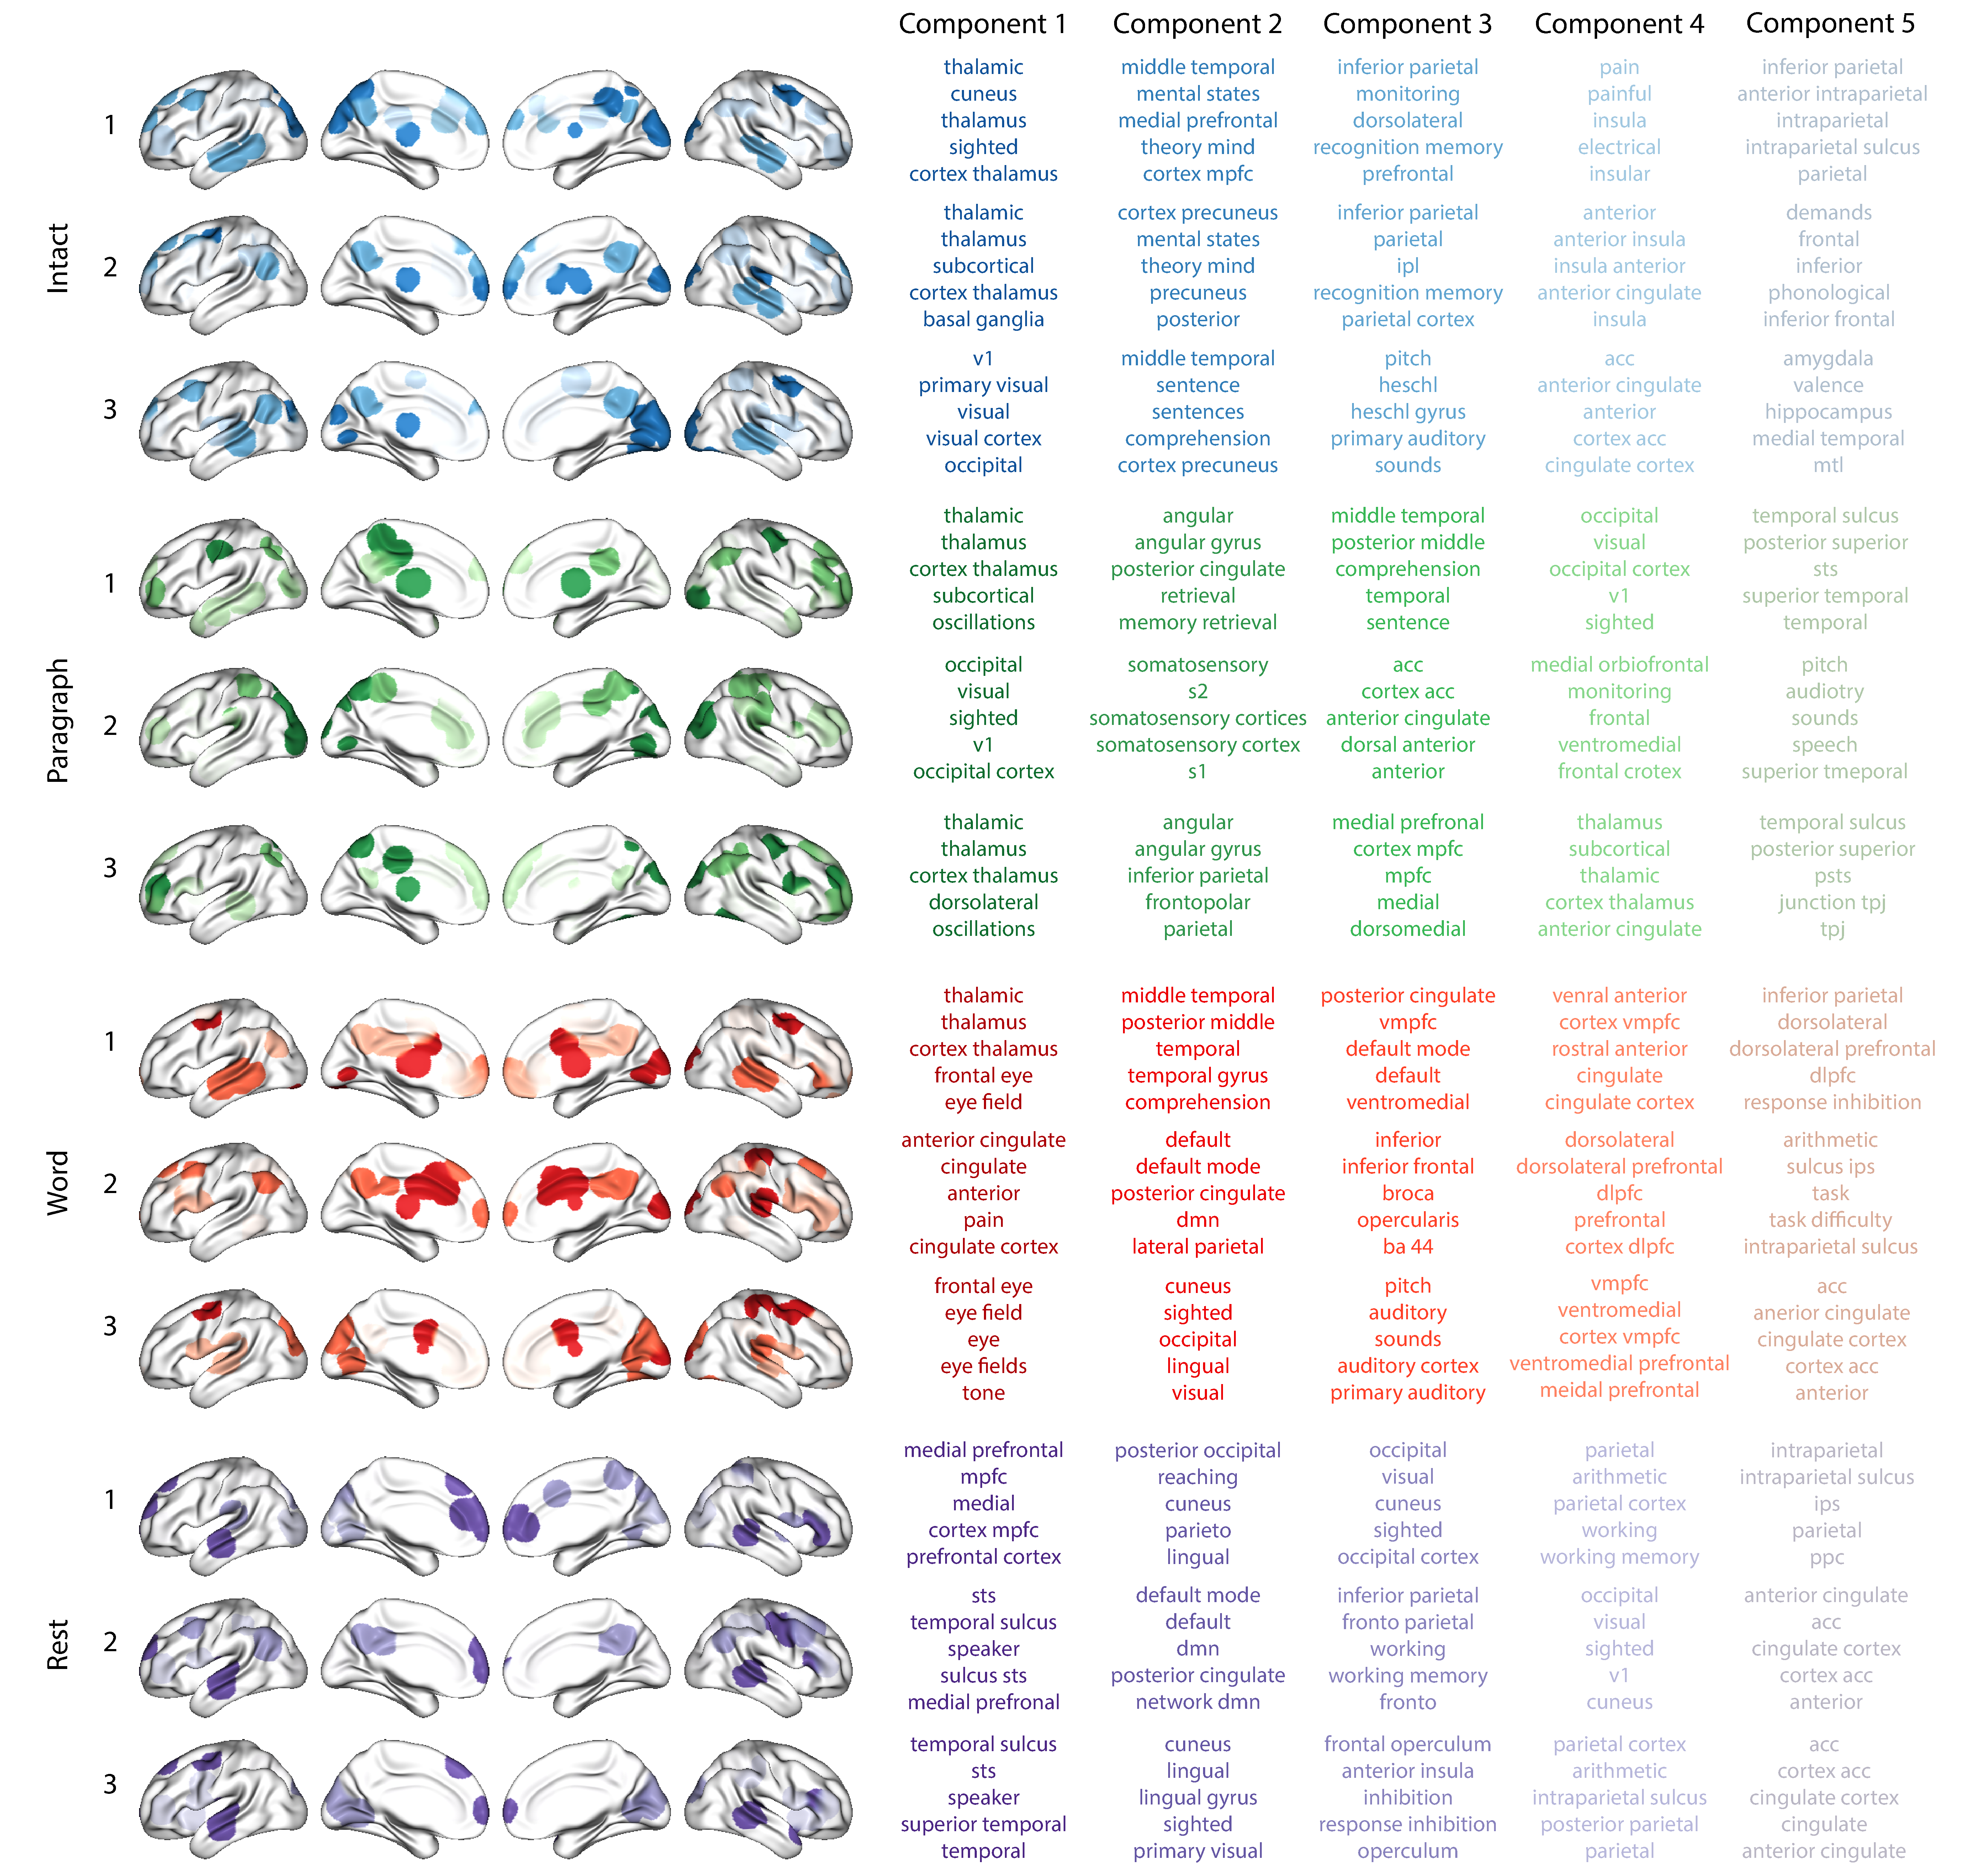
\includegraphics[width=\textwidth]{figs/pca_neurosynth_thirds}

\caption{\textbf{Top terms associated with the highest-weighted components by
condition, broken down by story segment.} Each group of three rows corresponds
to an experimental condition, and the colors correspond to the component number
(ranked by proportion of variance explained). The rows' numbering denotes the
story segment used to compute each map (1: first third; 2: second third; 3:
third third). The inflated brain plots display the top 20 highest-weighted hubs
(see \textit{Topographic Factor Analysis}) for each components. The lists on
the right display the top five Neurosynth terms~\citep{RubiEtal17} decoded from
each components' brain map. Analogous maps computed for the entire story may be
found in Figure~\synth.}

\label{fig:neurosynth-thirds}

\end{figure}

\include{figs/source/top_terms.tex}

\newpage
\renewcommand{\refname}{Supplemental references}
\bibliographystyle{apacite}
\bibliography{CDL-bibliography/cdl}

\end{document}


